\section{Dark-field microscopy}
\label{sec:DarkFMicro}

The following section explains the set-up for dark field microscopy and the process of adjustment. 

\subsection{Setup}

The setup itself consist of a system of lenses, a light source one mask and one camera as schematically depicted in \cref{fig:DarkFMicro}.
The way the microscope works is explained in section (ref). In our case all components were realized in a plug system of ThorLabs. We used a white LED as light source and a weak LASER to improve our adjustment of the setup. 
The setup is briefly introduced by following the path of the light. 

\begin{figure}[ht]
    \centering
    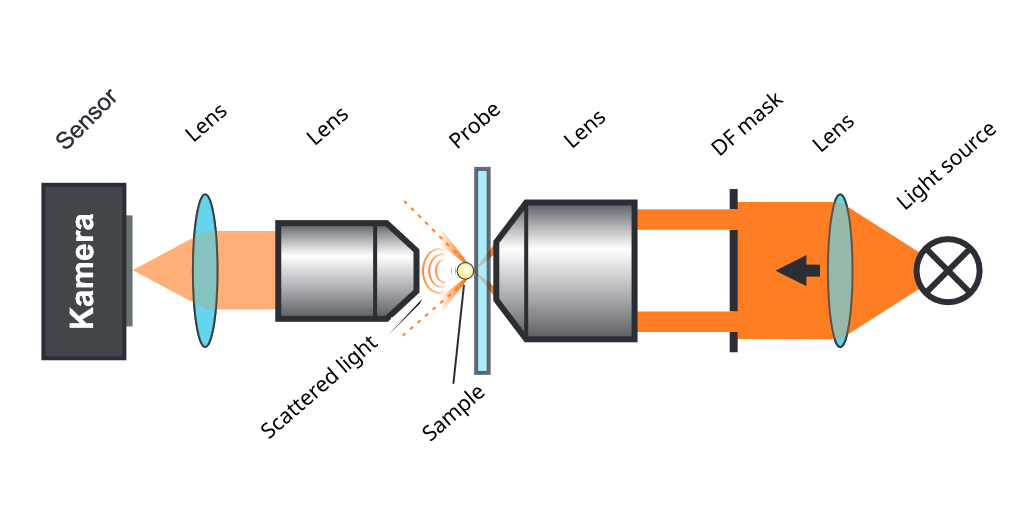
\includegraphics[width = \linewidth]{Bilder/Setup/MikroskopEdit.png}
    \caption{Schematic representation of the used dark-field microscope.}
    \label{fig:DarkFMicro}
\end{figure}

The first lense parallelizes the light. After this a dark field mask (DF mask) blocks the light which would directly enter in teh second lense of the microscope. The light which is transmitted by the DF mask is guided onto the sample and 
is scattered by the structure. This scattered light is picked up by the lense after the sample and converted to an image using the rest of the lenses. This picture is captured by the camera.

\subsection{Adjusting the setup}

The adjustment of the setup is performed in several steps. First the position of the first lens in adjusted, afterwards the second lense in focused on the sample and afterwards, the beam is guided into the spectrometer using two mirrors.

For 